\section{注意力模型}
注意力模型最近几年在深度学习各个领域被广泛使用, 无论是图像处理, 语音识别还是自然语言处理的各种不同类型的任务中, 都很容易遇到注意力模型的身影. 所以, 了解注意力机制的工作原理对于关注深度学习技术发展的技术人员来说有很大的必要. 

\subsection{算法流程}
以长度为4的序列为例, 解释注意力模块
\begin{figure}[!htbp]
    \centering
    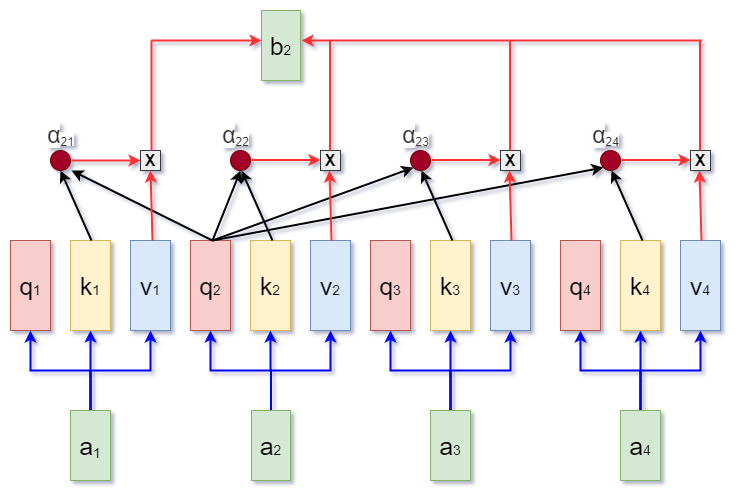
\includegraphics[height=22em]{pic/pic0101.png}
    \caption{注意力模型}
    \label{fig:0101}
\end{figure}

如~\ref{fig:0101}所示, 注意力模块的输入为序列$a_{1}, a_{2}, a_{3}, a_{4}$, 输出为$a_{2}$所对应的$b_{2}$. 其中$query$, $key$, $value$ 向量分别如~\ref{eq:0101}, ~\ref{eq:0102}所示.

\begin{equation}
    query_{i} = W^{q} a_{i}
    \label{eq:0101}
\end{equation}

\begin{equation}
    key_{i} = W^{k} a_{i}
    \label{eq:0102}
\end{equation}

对于每个注意力值 $\alpha_{i,j}$ 
\begin{equation}
    \alpha_{i,j} = query_{i} \cdot key_{j}
    \label{eq:0103}
\end{equation}

通过~\ref{eq:0104}得到$value$
\begin{equation}
    value_{i} = W^{v} a_{i}
    \label{eq:0104}
\end{equation}
将每个$value_{i}$和注意力值数值并累加, 可得到最终输出$b_{i}$
\begin{equation}
    b_{i} = \sum_{i, j} \alpha_{i,j} v_{j}
    \label{eq:0105}
\end{equation}

\subsection{矩阵形式}
将上述公式写为矩阵形式:
\begin{align*}
    query_{1} &= W^{q}\ a_{1}\\
    query_{2} &= W^{q}\ a_{2}\\
    query_{3} &= W^{q}\ a_{3}\\
    query_{4} &= W^{q}\ a_{4}\\
    [query_{1}\, query_{2}\, query_{3}\, query_{4}] & = W^{q} [a_{1}\, a_{2}\, a_{3}\, a_{4}]
\end{align*}
将所有输入$a_{i}$的集合写成$I$, 所有$query$的集合写成矩阵$Q$, 则:
\begin{equation}
    Q = W^{q}\; I
    \label{eq:0106}
\end{equation}

同理, $K=W^{k}\; I$, $V=W^{v}\; I$. 根据~\ref{eq:0103}, $query$ 要和 $key$ 做内积, 则可得, 注意力矩阵$A$为:
\begin{equation}
    A = QK^{T}
    \label{eq:0107}
\end{equation}
一般注意力模块中, 会将注意力矩阵$A$经过softmax操作得到$A^{\prime}$, 之后输出矩阵$B$为:
\begin{align}
    B &= A^{\prime}\ V\\
    B &= softmax(QK^{T})V
    \label{eq:0108}
\end{align}

注意~\ref{eq:0108}中矩阵的维度. $I_{mn}$, $Q_{mn}$, $K_{mn}$, $V_{mn}$, 而转换矩阵维度都为$W_{mm}$, 最后输出$B_{mn}$维度与输入矩阵$I_{mn}$相同. 网络要估计的参数为三个转换矩阵$W$

\subsection{算法思想}
将输入元素想象成是由一系列的<Key,Value>数据对构成, 此时给定某个元素Query,通过计算Query和各个Key的相似性或者相关性, 得到每个Key对应Value的权重系数, 然后对Value进行加权求和, 即得到了最终的Attention数值. 所以本质上Attention机制是对输入的Value值进行加权求和, 而Query和Key用来计算对应Value的权重系数. 

除了自注意力机制外, 还有通道维度增加注意力机制. 关键操作为squeeze和excitation, 所以论文将此attention结构命名为SE Block, SE Block显示实现特征通道的互相依赖关系, 获取到每个特征通道的重要程度, 然后用这个重要程度去给每一个特征通道赋予一个权值, 从而让神经网络重点关注某些特征通道, 提升对当前任务有用的特征通道, 并抑制对当前任务用处不大的特征通道. 
\begin{figure}[!htbp]
    \centering
    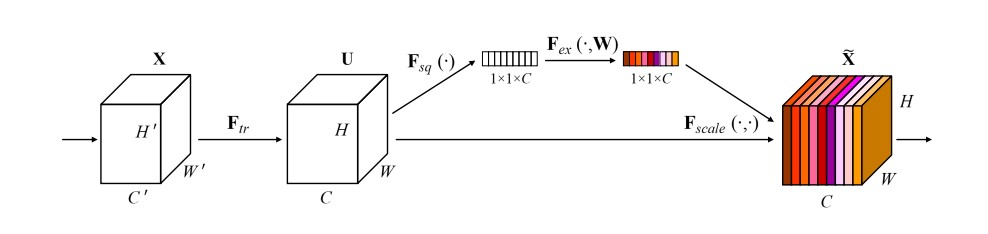
\includegraphics[height=8em]{pic/pic0102.jpg}
    \caption{通道注意力机制}
    \label{fig:0102}
\end{figure}

其具体实现如~\ref{fig:0103}所示, 通过两个FC和中间的ReLU激活函数找到了不同特征层之间的相互联系. 
\begin{figure}[!htbp]
    \centering
    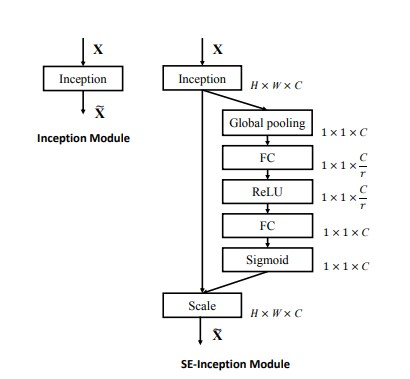
\includegraphics[height=12em]{pic/pic0103.jpg}
    \caption{SE Block}
    \label{fig:0103}
\end{figure}

% \begin{figure}[!htbp]
%     \centering
%     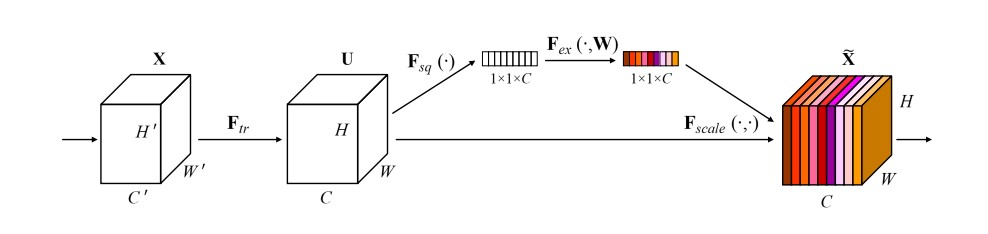
\includegraphics[height=22em]{pic/pic0102.jpg}
%     \caption{Quora 问答}
%     \label{fig:0102}
% \end{figure}

